\documentclass[
    a4paper,
    twocolumn,
    aps, pra,
    superscriptaddress,
    amsmath,amssymb
]{revtex4-2}

\usepackage{graphicx}
\usepackage{amsthm}
\usepackage{commath,mathtools}

\usepackage[caption=false]{subfig}

\usepackage[english]{babel}
\usepackage{fancyhdr}
\pagestyle{fancy}

\renewcommand\thesection{\Roman{section}}
\renewcommand\thesection{\arabic{section}}

\newtheorem{theorem}{Theorem}[section]
\newtheorem{lemma}[theorem]{Lemma}

\theoremstyle{definition}
\newtheorem{definition}[theorem]{Definition}

\newcommand{\fdOutside}[3]{\left(\pd{#1}{#2}\right)_{#3}}
\newcommand{\fd}[1]{\fdOutside #1}

\newcommand{\DeltaF}{\left.\Delta F\right|_T}
\newcommand{\DeltaS}{\left.\Delta S\right|_T}
\newcommand{\DeltaU}{\left.\Delta U\right|_T}

\lhead{Kom bij de \TeX niCie!}

\begin{document}
\title{Lorem ipsum dolor sit amet}

\author{Consectetur Adipiscing}
\affiliation{Department of Physics, Utrecht University}

\author{Morbi Quis}
\affiliation{Department of Physics, Utrecht University}

\begin{abstract}
    Cras luctus imperdiet viverra. In interdum egestas est ac pharetra. Sed consectetur, magna eu
    semper tempor, nisl massa pretium ante, quis varius elit mauris non turpis. Aenean bibendum
    consequat augue, non suscipit dolor interdum non. Vivamus facilisis, justo non fermentum
    ullamcorper, augue lorem varius justo, ut interdum odio enim ut sem.
\end{abstract}

\maketitle

\section{Introduction}

Vestibulum commodo luctus dui ut accumsan. Etiam non consectetur diam. Nam euismod ullamcorper
luctus. Mauris non nisi quam. Morbi ultrices nec nulla eu pulvinar. Phasellus aliquet sapien nec
libero consequat, vitae lacinia elit tristique.

\subsection{Eu rhoncus tellus luctus eu}

\begin{figure}
    \hfill\subfloat[]{%
        \includegraphics[width=0.45\linewidth]{example-image-a}%
        \label{fig:img-a}%
    }\hfill
    \subfloat[]{%
        \includegraphics[width=0.45\linewidth]{example-image-b}%
        \label{fig:img-b}%
    }\hfill\kern 0pt\relax
    \caption{Cras gravida nisl sapien, eu convallis urna auctor et. (a) Etiam eget congue mi.
    (b) Sed sit amet congue orci.}\label{fig:img-letters}
\end{figure}

Etiam condimentum laoreet velit fermentum molestie. Morbi posuere libero
facilisis lorem vulputate pulvinar. Integer venenatis quam ac sapien pellentesque varius. Morbi
vitae vestibulum metus. Nam gravida lacinia tortor. Maecenas hendrerit nulla sit amet
scelerisque aliquam, see Figure~\ref{fig:img-a}.

% \begin{theorem}
%     Quisque et justo hendrerit, auctor.
%     \begin{proof}
%         %Sodales felis,
%         Proin sodales tincidunt arcu,
%         \begin{align*}
%             \cos(2\theta) &= \cos^2(\theta) - \sin^2(\theta)\\
%             &= 2\cos^2(\theta) - 1,
%         \end{align*}
%         quis sagittis ipsum suscipit quis.
%     \end{proof}
% \end{theorem}

\begin{definition}
    Proin sodales tincidunt arcu,
    \begin{align*}
        \cos(2\theta) &= \cos^2(\theta) - \sin^2(\theta)\\
        &= 2\cos^2(\theta) - 1,
    \end{align*}
    quis sagittis ipsum suscipit quis.
\end{definition}

Nam, cum Figure~\ref{fig:img-letters}, vestibulum nibh hendrerit
consectetur tristique. Proin sodales tincidunt arcu, quis sagittis ipsum suscipit quis. Donec
dignissim mi odio, vel aliquam odio aliquam vitae.
% Vivamus nunc odio, imperdiet non pellentesque
% et, facilisis ac magna. Integer tincidunt nisl eu tellus gravida rutrum. Mauris eleifend ante
% urna, nec tincidunt augue commodo et. Aliquam pretium velit eget convallis tristique.

\section{Theory}

Praesent mauris augue, eleifend nec urna a, sodales maximus leo. Nam porta massa eu arcu
bibendum, vel scelerisque dui viverra. Aenean maximus, dui suscipit tincidunt efficitur, odio
elit rutrum mi, eget placerat orci libero id erat.

For the difference in entropy $ \DeltaS $ we derive
\begin{align*}
    \DeltaS &= \int \fd{SLT}\dif L = -\int \fd{fTL}\dif L,
\end{align*}
for the last step see eqn. 17.10 in \cite[][p. 193]{blundell}.

Suspendisse non ipsum consequat, porttitor
purus at, mattis enim. Fusce eleifend aliquam arcu vel pulvinar. Vestibulum augue felis,
tincidunt sit amet tristique quis, convallis vitae risus.

By definition of Helmholtz free energy we know $ F = U-TS $, meaning we can obtain $ \DeltaU $ as
\begin{align*}
\DeltaU = \DeltaF + T\DeltaS.
\end{align*}
Sed porta, lorem vitae venenatis imperdiet, massa velit sollicitudin tellus, in lacinia enim ex
euismod lorem.

% Mauris viverra, nulla et venenatis faucibus, erat dolor blandit
% justo, eu aliquam urna felis sed dolor. Vestibulum eu nisi sit amet ex tincidunt eleifend. Nam
% nunc ante, cursus in lobortis sit amet, cursus eu ex. Donec suscipit euismod risus lacinia
% gravida.

\section{Setup and method}

\newsavebox{\setupExpl}
\sbox{\setupExpl}{%
	\parbox{\columnwidth}{%
		\begin{enumerate}
            \setlength{\itemsep}{0pt}
		    \setlength{\parskip}{0pt}
			\item Rubber band submerged in water column, fixed to the bottom of the column and fixed to the sensor part of element 2.
			\item Force sensor, fixed to element 3.
			\item Device fixing the force sensor to a certain height.
			\item Heatbath water reservoir which can be set to different temperatures and will pump it through the water column to maintain a uniform temperature.
		\end{enumerate}
	}\newline
}

\begin{figure}[h]
	\centering
	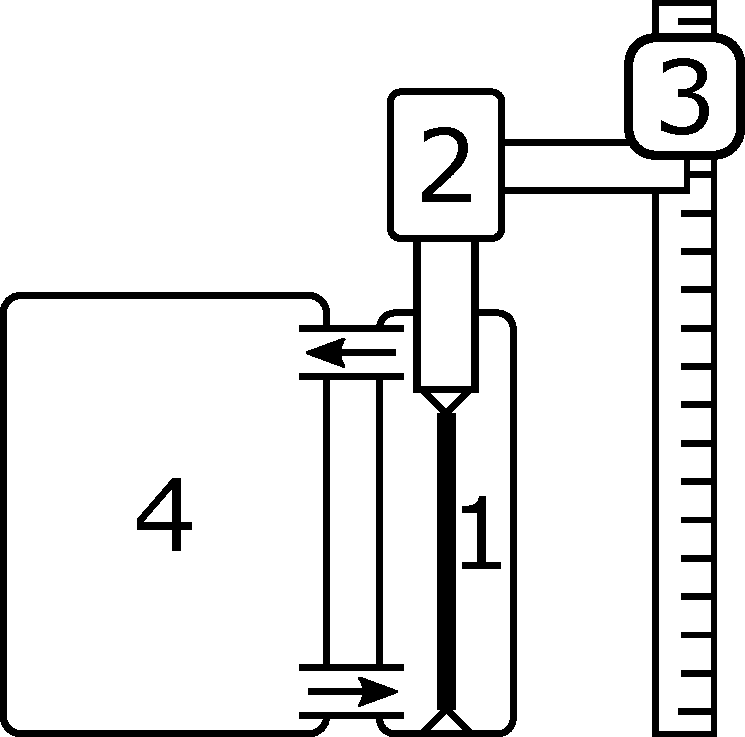
\includegraphics[width=0.2\textwidth]{assets/OpstellingTekening1.pdf}
	\caption[Diagram of the measurement setup]{
        Diagram of the measurement setup. The elements are\newline
        \usebox{\setupExpl}}\label{fig:setupSchematic}
    \rule{0.5\linewidth}{1pt}
\end{figure}

Etiam et mollis ante, ac consequat risus. Suspendisse convallis a enim vitae laoreet. Nam
sagittis auctor felis. Nunc feugiat purus lorem, in pulvinar leo accumsan quis. Maecenas
tristique sollicitudin venenatis. Phasellus imperdiet urna quis augue ornare condimentum. Cras
euismod nisi convallis ipsum ultricies aliquet.
Suspendisse accumsan vulputate accumsan. Aliquam
vehicula sapien quis egestas venenatis. Nam suscipit imperdiet eros eget finibus. Interdum et
malesuada fames ac ante ipsum primis in faucibus. Quisque porta ultricies eros nec posuere. In
hendrerit eleifend nisl a volutpat. Suspendisse pharetra diam non leo efficitur pretium. Ut sed
dolor tincidunt sem vulputate elementum. Curabitur odio felis, accumsan eu sollicitudin vitae,
tempus sit amet velit.

Pellentesque lobortis sagittis fermentum. Praesent finibus euismod ex, nec rhoncus metus
pulvinar quis. Cras sed lectus augue. Pellentesque habitant morbi tristique senectus et netus et
malesuada fames ac turpis egestas. Cras a convallis mi, a finibus felis. Nunc quis nisi non
magna tincidunt tincidunt. Maecenas cursus, velit non dapibus gravida, quam dui condimentum leo,
ac egestas tellus sem a est. Pellentesque convallis sollicitudin commodo. Nulla non viverra
sapien.

Etiam sit amet neque rutrum, semper ex et, vehicula diam. Aliquam iaculis dignissim accumsan.
Integer vel suscipit ligula, at efficitur nulla. Proin iaculis quam at mattis bibendum. Vivamus
mauris enim, convallis sit amet massa at, venenatis luctus diam. Curabitur vel vehicula turpis.
Nulla blandit, augue quis pharetra posuere, sem justo vehicula nibh, quis tempus felis magna blandit
augue. Morbi non blandit tellus. Cras aliquet nulla nisl, sed elementum tortor imperdiet ut. Integer
volutpat, nibh sed vehicula vestibulum, felis orci euismod sapien, sed ullamcorper lorem metus vel
ligula.

\addcontentsline{toc}{section}{Bibliography}
\begin{thebibliography}{10}

\bibitem{young_wiki} Young's modulus - Wikipedia. 2019. [accessed 2019 Oct 25].  \url{https://en.wikipedia.org/wiki/Young's_modulus#Approximate_values}.

\bibitem[Blundell et al.(2010)S.J.~Blundell and K.M.~Blundell]{blundell}
S.J.~Blundell, and K.M.~Blundell, \textit{Concepts in Thermal Physics, Second edition} (Oxford University Press Inc., New York, 2010).

\end{thebibliography}

\end{document}
